\documentclass[12pt,a4paper]{report}
% --- Packages ---
\usepackage[utf8]{inputenc}
\usepackage[T1]{fontenc}
\usepackage{geometry}
\geometry{margin=1in}
\usepackage{graphicx}
\usepackage{booktabs} % For professional tables
\usepackage{hyperref} % For clickable links
\usepackage{titlesec} % For custom chapter titles
\usepackage{listings} % For code snippets
\usepackage{xcolor}
\usepackage{tikz}
\usepackage{pgf-pie}
\usepackage{subcaption}
\usepackage{float}
\usetikzlibrary{shapes.geometric, arrows, positioning, fit, backgrounds}
% Define styles for diagrams
\tikzstyle{server} = [rectangle, rounded corners , minimum width=3cm, minimum height=1cm, text centered, draw=black, fill=blue!30]
\tikzstyle{client} = [rectangle, rounded corners, minimum width=2.5cm, minimum height=0.8cm, text centered, draw=black, fill=green!30]
\tikzstyle{database} = [cylinder, shape border rotate=90, aspect=0.25, minimum width=2cm, minimum height=1.5cm, draw=black, fill=orange!30]
\tikzstyle{arrow} = [thick,->,>=stealth]
% --- Settings ---
\hypersetup{colorlinks=true, linkcolor=blue, urlcolor=cyan}
\lstset{basicstyle=\ttfamily\small, breaklines=true, frame=single}
% --- Document Start ---
\begin{document}
% --- Title Page ---
\begin{titlepage}
    \centering
    \vspace*{1cm}
    {\huge \textbf{MangaHub: A Multi-Protocol Network Programming System}} \\
    \vspace{0.5cm}
    {\large Net-Centric Programming Project Report} \\
    \vspace{1.5cm}

    % University Logo
    \includegraphics[width=0.5\textwidth]{figures/logo.png} \\
    \vspace{1cm}

    {\large \textbf{IT096IU - Net-Centric Programming}} \\
    \vspace{0.5cm}
    {\large Instructor: Dr. Le Thanh Son} \\
    \vfill
    A project report submitted in partial fulfillment of the requirements for \\
    the Net-Centric Programming course (IT096IU) \\
    \vspace{0.8cm}
    Department of Computer Science \\
    International University \\
    Vietnam National University - Ho Chi Minh City \\
    \vspace{0.5cm}
    \today
\end{titlepage}
% --- Front Matter ---
\pagenumbering{arabic}
\setcounter{page}{1}
\tableofcontents
\listoffigures
\listoftables
\chapter*{Contribution Table}\addcontentsline{toc}{chapter}{Contribution Table}
\begin{table}[htbp]
    \centering
    \begin{tabular}{|l|l|p{9cm}|} % Added an extra 'l' for the ID column
        \hline
        \textbf{Member Name} & \textbf{ID} & \textbf{Contribution} \\ \hline
        Tran Nguyen Phuc & ITCSIU21097 & Backend development (HTTP API, TCP Server, UDP Server), Database design and implementation, Testing and quality assurance, Deployment and DevOps, Report writing (Chapters 3-5) \\ \hline
        Nguyen Mach Khang Huy & ITCSIU21072 & Frontend development (Next.js, WebSocket integration), gRPC service implementation, System architecture documentation, Report writing (Chapters 1-2, 6) \\ \hline
    \end{tabular}
    \caption{Project Contribution Summary}
\end{table}

\chapter*{Abstract}\addcontentsline{toc}{chapter}{Abstract}
MangaHub is a comprehensive network programming project developed as part of the IT096IU Net-Centric Programming course at International University, Vietnam National University - Ho Chi Minh City. The system demonstrates the practical implementation of five major network protocols: HTTP, TCP, UDP, WebSocket, and gRPC, integrated into a unified manga and comic tracking application.

The project addresses the real-world challenge of tracking manga reading progress across multiple devices and platforms. Through a client-server architecture built with Go programming language, the system enables users to manage their manga library, synchronize reading progress in real-time, receive notifications about new chapter releases, and participate in community discussions.

The HTTP REST API server handles user authentication, manga catalog management, and library operations. The TCP synchronization server ensures real-time progress updates across all connected devices using JSON-based messaging. UDP broadcasts deliver instant chapter release notifications to subscribed clients. WebSocket technology powers the real-time chat system for manga discussions, while gRPC facilitates efficient internal service-to-service communication.

The system employs modern software engineering practices including clean architecture, concurrent programming with goroutines, JWT-based authentication, and comprehensive testing strategies. A Next.js web frontend provides an intuitive user interface, while a command-line tool offers advanced functionality for power users. This report presents a detailed examination of the project's design, implementation, testing, and deployment, demonstrating how multiple network protocols can be integrated cohesively to create a practical, scalable, and user-friendly application.
\clearpage\chapter{Introduction}

\section{Project Background and Motivation}
The digital consumption of manga and comics has experienced exponential growth in recent years, with millions of readers worldwide accessing content across multiple platforms and devices. However, this proliferation has created a significant challenge: readers often lose track of their progress when switching between devices, struggle to stay updated on new chapter releases, and lack effective tools for organizing their extensive reading lists.

Network programming forms the backbone of modern distributed systems, enabling seamless communication between clients and servers across the internet. Understanding how different network protocols work together to create cohesive applications is essential for computer science students preparing for careers in software development, cloud computing, and systems engineering.

MangaHub was conceived to address both challenges simultaneously. By building a practical manga tracking system, the project demonstrates how multiple network protocols can work together to solve real-world problems. The application requires HTTP for RESTful API operations, TCP for reliable real-time synchronization, UDP for broadcast notifications, WebSocket for bidirectional communication, and gRPC for efficient inter-service communication. The choice of Go (Golang) as the primary programming language was motivated by its excellent support for concurrent programming, built-in networking capabilities, and growing adoption in cloud-native applications.

\section{Objectives}
The primary objective of this project is to demonstrate comprehensive understanding of network programming concepts through practical implementation of five major network protocols. Each protocol was carefully selected to address specific requirements of the manga tracking system while providing educational value in understanding their strengths, limitations, and appropriate use cases. The specific objectives include:
\begin{itemize}
    \item \textbf{Implement HTTP REST API:} Design and develop a complete RESTful API server supporting user authentication, CRUD operations for manga management, library management, and reading progress tracking. The API follows REST architectural principles, implements proper HTTP status codes, and provides comprehensive error handling with standardized response formats.
    \item \textbf{Build TCP Synchronization Server:} Create a TCP server that maintains persistent connections with clients to enable real-time synchronization of reading progress across multiple devices. The implementation handles concurrent connections efficiently using goroutines and implements a robust JSON-based messaging protocol with acknowledgment mechanisms.
    \item \textbf{Develop UDP Notification Service:} Implement a UDP broadcast system for sending chapter release notifications to subscribed clients. The system handles client registration, maintains subscription lists, and efficiently broadcasts updates without guaranteeing delivery order, demonstrating UDP's best-effort delivery model.
    \item \textbf{Create WebSocket Chat System:} Build a real-time chat application using WebSocket protocol, supporting multiple chat rooms, user presence detection, and message broadcasting. The system handles connection upgrades from HTTP and manages room-based message routing efficiently.
    \item \textbf{Implement gRPC Internal Service:} Design and implement gRPC services for internal communication between system components, utilizing Protocol Buffers for efficient data serialization. The implementation demonstrates both unary and streaming RPC patterns, showcasing gRPC's type safety and performance benefits.
\end{itemize}

\section{Project Scope}
The MangaHub project encompasses a comprehensive set of features designed to demonstrate network programming concepts while providing practical functionality. The scope has been carefully defined to balance educational objectives with project feasibility within the course timeline. The following sections detail what is included and explicitly excluded from the project.

\subsection{In Scope}
The project includes five independent server processes implementing HTTP (port 8080), TCP (port 9090), UDP (port 9091), WebSocket (via HTTP upgrade), and gRPC (port 9092) protocols. User authentication and authorization is implemented using JWT tokens with bcrypt password hashing. The system provides a complete manga catalog with search and filtering capabilities, personal library management for organizing collections, and real-time progress synchronization across multiple client connections. Chapter release notifications are broadcast via UDP to subscribed clients. Multi-room chat functionality enables manga-specific discussions and a general community chat. The SQLite database includes a migration system for schema versioning. A web frontend built with Next.js, TypeScript, and Tailwind CSS provides an intuitive interface, while a command-line tool offers advanced functionality. Comprehensive API documentation, unit and integration testing suites, and Docker containerization complete the deliverables.

\subsection{Out of Scope}
The project explicitly excludes actual manga reading functionality (viewing pages), payment processing or subscription management, social features beyond basic chat (friend systems, user profiles), mobile native applications, content recommendation algorithms, advanced analytics or reporting features, multi-language internationalization support, and production-grade scalability optimizations. These exclusions allow the team to focus on core network programming demonstrations while maintaining a realistic project scope.

\section{Tools and Technologies}
The MangaHub project leverages modern development tools and technologies selected for their suitability to network programming education and real-world applicability. Each tool was chosen based on its strengths in demonstrating specific concepts, community support, documentation quality, and industry relevance.
\begin{itemize}
    \item \textbf{Go (Golang) 1.19+}: Serves as the primary backend language, chosen for its exceptional concurrency model with goroutines and channels.
    \item \textbf{TypeScript 5.0+}: Used for frontend development, providing type safety and improved developer experience over JavaScript.
    \item \textbf{Gin Framework}: A high-performance HTTP web framework for building RESTful APIs in Go.
    \item \textbf{Gorilla WebSocket}: A battle-tested Go library for implementing WebSocket servers.
    \item \textbf{gRPC-Go}: The official Go implementation of gRPC for high-performance RPC.
    \item \textbf{Next.js 14}: A React framework for building server-side rendered and static web applications.
    \item \textbf{React 18}: A component-based UI library for building user interfaces.
    \item \textbf{Tailwind CSS 3}: A utility-first CSS framework for rapid UI development.
    \item \textbf{SQLite3}: An embedded relational database for simple, zero-configuration data storage.
    \item \textbf{Git/GitHub}: Distributed version control and collaboration platform.
    \item \textbf{Visual Studio Code}: The primary IDE with extensions for Go, ESLint, and Prettier.
    \item \textbf{Docker}: Containerization platform for packaging and deploying applications.
\end{itemize}% --- Chapter 2 ---\chapter{Literature Review}

\section{Network Programming Fundamentals}
Network programming forms the foundation of distributed systems, enabling communication between processes running on different machines across local or wide area networks. At its core, network programming involves creating applications that can send and receive data using various protocols and communication patterns.
\subsection{The OSI and TCP/IP Models}
The OSI (Open Systems Interconnection) model provides a seven-layer conceptual framework for network communications. However, practical implementations typically follow the simpler four-layer TCP/IP model: Network Access, Internet (IP), Transport (TCP/UDP), and Application (HTTP, etc.).
\subsection{Socket Programming}
A socket acts as an endpoint for sending or receiving data, identified by an IP address and port number. The Berkeley sockets API is the de facto standard, and Go's \texttt{net} package provides a high-level abstraction over these operations.
\subsection{Concurrency in Network Programming}
Concurrent programming is essential for handling multiple simultaneous connections. Go addresses the limitations of traditional threading with goroutines, which are lightweight threads (2KB initial stack) managed by the Go runtime, enabling efficient handling of thousands of connections.

\section{TCP/IP Protocol Suite}
\subsection{TCP (Transmission Control Protocol)}
TCP provides reliable, ordered, and error-checked delivery of data. It establishes connections via a three-way handshake (SYN, SYN-ACK, ACK), implements flow and congestion control, sequences and acknowledges every byte, and terminates connections gracefully with a four-way handshake.
\subsection{UDP (User Datagram Protocol)}
UDP offers a connectionless, best-effort delivery service. It is faster but less reliable than TCP, as packets may be lost, duplicated, or arrive out of order. Its low latency makes it suitable for real-time applications like video streaming, gaming, and broadcast notifications.
\subsection{The IP Layer and Port Numbers}
The Internet Protocol (IP) handles routing packets using IP addresses (32-bit for IPv4, 128-bit for IPv6). Port numbers (16-bit) differentiate services on a single host.

\section{HTTP and RESTful Architecture}
The Hypertext Transfer Protocol (HTTP) is a request-response protocol that forms the foundation of the web.
\subsection{REST Principles}
Representational State Transfer (REST) is an architectural style that treats resources as entities identified by URIs. Key principles include client-server separation, statelessness, cacheability, and a uniform interface using standard HTTP methods (GET, POST, PUT, PATCH, DELETE).
\subsection{HTTP Status Codes}
Status codes provide standardized responses: 2xx for success, 3xx for redirection, 4xx for client errors (e.g., 404 Not Found, 401 Unauthorized), and 5xx for server errors.

\section{WebSocket Real-time Communication}
WebSocket provides full-duplex communication channels over a single TCP connection, enabling bidirectional data flow ideal for real-time applications.
\subsection{The WebSocket Protocol}
A WebSocket connection begins with an HTTP "Upgrade" request. Once established, data is transmitted in frames. The protocol supports text and binary data, fragmentation, and ping/pong keepalive messages. WSS (WebSocket Secure) provides encryption.
\subsection{Comparison with Alternatives}
Compared to Long Polling or Server-Sent Events (SSE), WebSocket offers true bidirectional communication with lower latency and overhead, making it superior for applications like live chat and real-time notifications.

\section{gRPC and Protocol Buffers}
gRPC is a high-performance Remote Procedure Call (RPC) framework from Google that uses HTTP/2 for transport and Protocol Buffers for serialization.
\subsection{Protocol Buffers (Protobuf)}
Protobuf is a language-neutral mechanism for serializing structured data into an efficient and compact binary format. It is smaller and faster than JSON or XML and provides strong typing and schema evolution.
\subsection{gRPC vs. REST}
gRPC offers superior performance, streaming capabilities, and strong typing, making it ideal for internal microservice communication. REST provides broader compatibility (especially in browsers) and is more human-readable. In MangaHub, gRPC is used for internal services, while a REST API serves external clients.% --- Chapter 3 ---\chapter{System Design and Architecture}

\section{System Architecture Overview}
The MangaHub system is designed as a microservices-style application, with a backend built entirely in Go (Golang). The architecture is centered around five distinct, independently deployable services, each responsible for a specific network protocol. This separation of concerns allows for clear protocol demonstration, fault isolation, and independent scalability.

\begin{figure}[htbp]
    \centering
    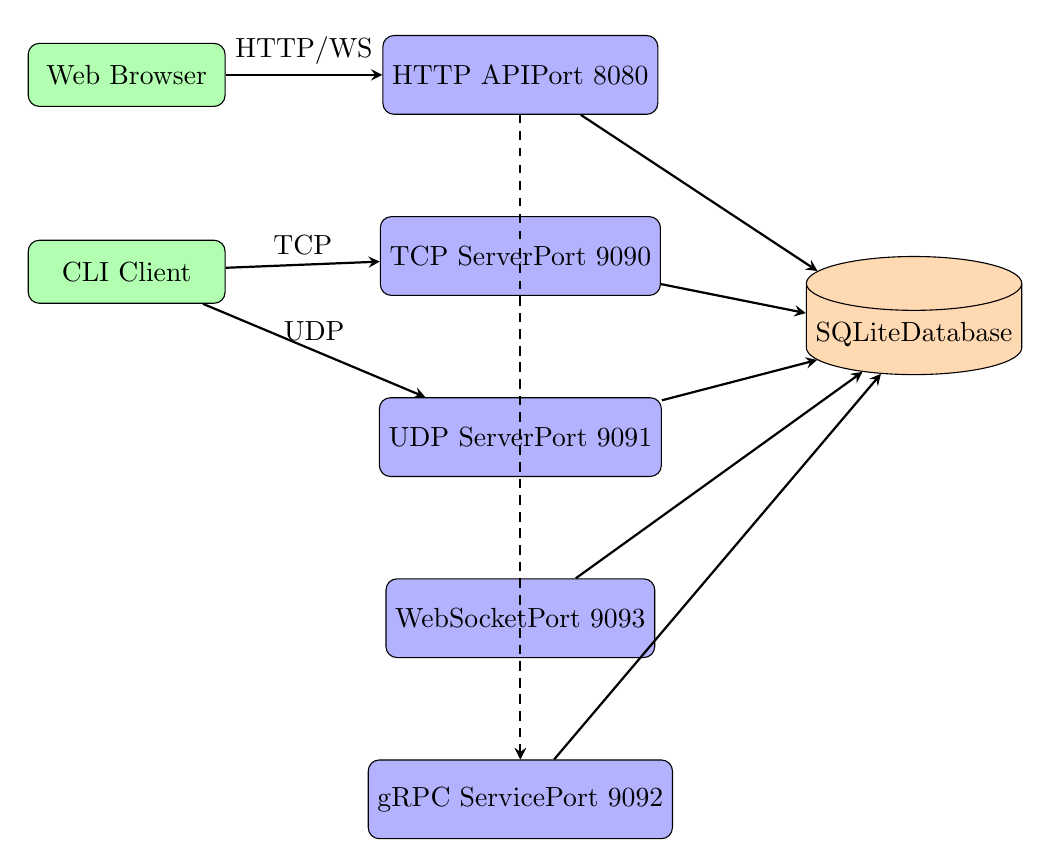
\begin{tikzpicture}[node distance=2cm]
        % Clients
        \node (web) [client] {Web Browser};
        \node (cli) [client, below of=web, yshift=-0.5cm] {CLI Client};

        % Servers
        \node (http) [server, right of=web, xshift=3cm] {HTTP API\\Port 8080};
        \node (tcp) [server, below of=http, yshift=-0.3cm] {TCP Server\\Port 9090};
        \node (udp) [server, below of=tcp, yshift=-0.3cm] {UDP Server\\Port 9091};
        \node (ws) [server, below of=udp, yshift=-0.3cm] {WebSocket\\Port 9093};
        \node (grpc) [server, below of=ws, yshift=-0.3cm] {gRPC Service\\Port 9092};

        % Database
        \node (db) [database, right of=tcp, xshift=3cm, yshift=-1cm] {SQLite\\Database};

        % Arrows
        \draw [arrow] (web) -- node[anchor=south] {HTTP/WS} (http);
        \draw [arrow] (cli) -- node[anchor=south] {TCP} (tcp);
        \draw [arrow] (cli) -- node[anchor=south] {UDP} (udp);

        \draw [arrow] (http) -- (db);
        \draw [arrow] (tcp) -- (db);
        \draw [arrow] (udp) -- (db);
        \draw [arrow] (ws) -- (db);
        \draw [arrow] (grpc) -- (db);

        \draw [arrow, dashed] (http) -- (grpc);
        \draw [arrow, dashed] (tcp) -- (grpc);
    \end{tikzpicture}
    \caption{MangaHub System Architecture Overview}
    \label{fig:architecture}
\end{figure}

The project follows the standard Go project layout to maintain a clean and organized codebase:
\begin{itemize}
    \item \textbf{/cmd}: Contains the main application entry points. Each of the five servers (API, TCP, UDP, WebSocket, gRPC) has its own subdirectory here, containing a `main.go` file responsible for starting that specific server.
    \item \textbf{/internal}: Houses the core business logic, services, and repositories. This code is private to the MangaHub project and cannot be imported by external applications, enforcing a clean separation between internal implementation and public-facing components.
    \item \textbf{/pkg}: Includes shared libraries and data models (e.g., `models.Manga`, `models.User`) that are safe to be used across different services within the project.
    \item \textbf{/proto}: Contains the Protocol Buffer (`.proto`) definitions for the gRPC service, which define the service contracts for internal RPC communication.
\end{itemize}

The five core services communicate with each other and with client applications as follows:
\begin{enumerate}
    \item \textbf{HTTP REST API Server (Port 8080)}: The primary entry point for client applications. Built with the Gin framework, it handles user authentication, manga library management, and CRUD operations. It communicates with the database via the repository layer.
    \item \textbf{TCP Sync Server (Port 9090)}: A custom TCP server for real-time synchronization of reading progress. Clients maintain a persistent connection to this server, which broadcasts updates to all connected devices for a given user.
    \item \textbf{UDP Notification Server (Port 9091)}: A custom UDP server that broadcasts new chapter release notifications to subscribed clients in a "fire-and-forget" manner.
    \item \textbf{WebSocket Chat Server (Port 9093)}: Handles real-time, multi-room chat. The connection is initiated via an HTTP upgrade request handled by the API server, after which communication is managed by a dedicated WebSocket hub using the Gorilla WebSocket library.
    \item \textbf{gRPC Internal Service (Port 9092)}: Uses gRPC-Go for efficient, type-safe communication between internal services, such as fetching user data or manga details without the overhead of a full HTTP request.
\end{enumerate}

\section{Database Design}
The system utilizes SQLite3 as its database, chosen for its simplicity, file-based nature, and lack of a required server process, making it ideal for a self-contained academic project. The database schema is managed through a versioned migration system located in the `/migrations` directory. Each migration is an SQL file that defines a specific schema change, allowing the database to be version-controlled and easily set up in new environments.

\begin{figure}[htbp]
    \centering
    \begin{tikzpicture}[node distance=3cm]
        % Users table
        \node (users) [rectangle, draw, align=left, fill=blue!10] {
            \textbf{USERS}\\
            \hline
            id (PK)\\
            username\\
            email\\
            password\_hash\\
            created\_at
        };

        % Manga table
        \node (manga) [rectangle, draw, align=left, fill=green!10, right of=users, xshift=2cm] {
            \textbf{MANGA}\\
            \hline
            id (PK)\\
            title\\
            author\\
            genres\\
            status\\
            total\_chapters
        };

        % User Progress table
        \node (progress) [rectangle, draw, align=left, fill=orange!10, below of=users, yshift=-1cm, xshift=2cm] {
            \textbf{USER\_PROGRESS}\\
            \hline
            user\_id (FK)\\
            manga\_id (FK)\\
            current\_chapter\\
            current\_page\\
            status\\
            rating
        };

        % Relationships
        \draw [arrow] (users) -- node[anchor=east] {1:M} (progress);
        \draw [arrow] (manga) -- node[anchor=west] {1:M} (progress);
    \end{tikzpicture}
    \caption{Database Entity-Relationship Diagram}
    \label{fig:er-diagram}
\end{figure}

The core database schema consists of the following tables:
\begin{itemize}
    \item \texttt{users}: Stores user information, including a unique ID, username, email, and a hashed password (using bcrypt).
    \item \texttt{manga}: Contains the catalog of all manga, with details such as title, author, genres, status, and cover image URL.
    \item \texttt{user\_progress}: A linking table that tracks the reading progress for each user and each manga, including the current chapter, reading status (e.g., 'reading', 'completed'), and rating.
\end{itemize}
This relational design allows for efficient querying of a user's library and progress.

\section{Network Protocol Implementation}
Each of the five network protocols is implemented in its own dedicated service to demonstrate a clear understanding of its use case.
\begin{itemize}
    \item \textbf{HTTP}: Implemented using the Gin web framework. The API follows RESTful principles, using standard HTTP methods (GET, POST, PUT, DELETE) and status codes. Routes are organized into groups, and middleware is used for logging, authentication (JWT), and error handling.
    \item \textbf{TCP}: A custom server built using Go's standard `net` package. It runs a loop to accept incoming connections, and each connection is handled in a separate goroutine for concurrency. A JSON-based messaging format is used for communication between the client and server.
    \item \textbf{UDP}: Also built using the `net` package. The server listens for datagrams on a specific port. It maintains a list of subscribed client addresses and broadcasts notification messages to all of them.
    \item \textbf{WebSocket}: Implemented using the popular Gorilla WebSocket library. An HTTP endpoint on the Gin server handles the initial "Upgrade" request. Once the connection is upgraded, it is handed off to a central "hub" that manages clients, rooms, and message broadcasting.
    \item \textbf{gRPC}: The service is defined in a `.proto` file, which specifies the RPC methods and message structures. The `protoc` compiler is used to generate Go code for the server and client stubs. The gRPC server is implemented to handle internal requests with high performance and type safety.
\end{itemize}

\section{Security Architecture}
Security is a key consideration in the MangaHub project. The following measures are implemented:
\begin{itemize}
    \item \textbf{Authentication}: User authentication is handled via JSON Web Tokens (JWT). When a user logs in, the server issues a signed JWT containing the user's ID. This token must be included in the `Authorization` header of subsequent requests to protected endpoints.
    \item \textbf{Password Hashing}: User passwords are never stored in plaintext. They are hashed using the \texttt{bcrypt} algorithm, which is a strong, adaptive hashing function that is resistant to brute-force attacks.
    \item \textbf{Secure Communication}: While not explicitly stated for all services in a development environment, production deployment would involve using TLS (Transport Layer Security) to encrypt all communication between clients and servers (HTTPS, WSS, etc.).
    \item \textbf{CORS}: Cross-Origin Resource Sharing (CORS) policies are configured in the Gin API server to control which domains are allowed to access the API, preventing malicious websites from making unauthorized requests.
\end{itemize}% --- Chapter 4 ---\chapter{Implementation}
This chapter details the specific implementation of each of the five network protocol servers and the web frontend. The code is structured to be modular and maintainable, with each server running as a separate process.

\section{HTTP REST API Server}
The HTTP server is built using the Gin web framework and serves as the main entry point for most client interactions.
\begin{itemize}
    \item \textbf{Entry Point}: The server is started from \texttt{cmd/api-server/main.go}. This file is responsible for initializing the database connection, setting up the Gin router, defining routes, and starting the HTTP listener on port 8080.
    \item \textbf{Routing and Middleware}: Routes are defined in a dedicated router function. They are grouped logically (e.g., \texttt{/auth}, \texttt{/manga}, \texttt{/users}). Middleware for JWT authentication, logging, and CORS is applied to the relevant route groups.
    \item \textbf{Handlers}: Handler functions, located in the \texttt{internal/handlers} directory, are responsible for processing incoming HTTP requests. They parse request bodies and parameters, call the appropriate service-layer functions to perform business logic, and return JSON responses with correct HTTP status codes. The "Handler -> Service -> Repository" pattern is followed to separate concerns.
\end{itemize}

\section{TCP Synchronization Server}
The TCP server provides real-time synchronization of a user's reading progress across multiple devices.
\begin{itemize}
    \item \textbf{Entry Point}: The server is launched from \texttt{cmd/tcp-server/main.go}, which starts a TCP listener on port 9090.
    \item \textbf{Connection Handling}: The server runs an infinite loop that accepts new TCP connections. Each incoming connection is handled in its own goroutine to allow for concurrent processing of multiple clients.
    \item \textbf{Messaging Protocol}: Upon connection, a client sends an authentication message (containing a JWT). The server maintains a map of authenticated connections. A simple JSON-based messaging protocol is used to send and receive progress updates. When a progress update is received from one client, the server broadcasts it to all other connected clients belonging to the same user.
\end{itemize}

\begin{figure}[htbp]
    \centering
    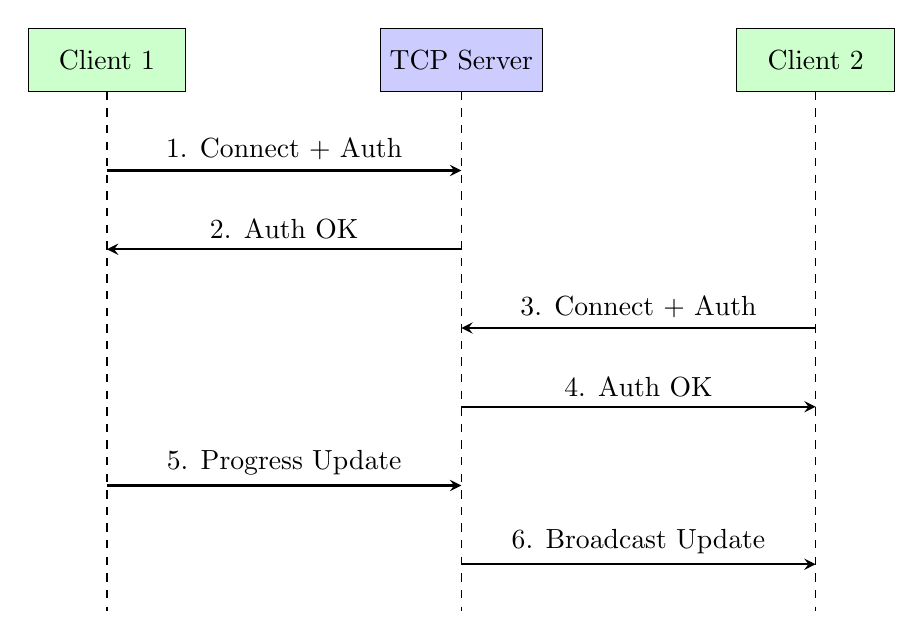
\begin{tikzpicture}[node distance=1.5cm]
        % Define styles for sequence diagram
        \tikzstyle{box} = [rectangle, draw, minimum width=2cm, minimum height=0.8cm]

        % Actors
        \node (client1) [box, fill=green!20] {Client 1};
        \node (server) [box, fill=blue!20, right of=client1, xshift=3cm] {TCP Server};
        \node (client2) [box, fill=green!20, right of=server, xshift=3cm] {Client 2};

        % Lifelines
        \draw [dashed] (client1) -- ++(0,-7);
        \draw [dashed] (server) -- ++(0,-7);
        \draw [dashed] (client2) -- ++(0,-7);

        % Messages
        \draw [arrow] ([yshift=-1cm]client1.south) -- node[above] {1. Connect + Auth} ([yshift=-1cm]server.south);
        \draw [arrow] ([yshift=-2cm]server.south) -- node[above] {2. Auth OK} ([yshift=-2cm]client1.south);

        \draw [arrow] ([yshift=-3cm]client2.south) -- node[above] {3. Connect + Auth} ([yshift=-3cm]server.south);
        \draw [arrow] ([yshift=-4cm]server.south) -- node[above] {4. Auth OK} ([yshift=-4cm]client2.south);

        \draw [arrow] ([yshift=-5cm]client1.south) -- node[above] {5. Progress Update} ([yshift=-5cm]server.south);
        \draw [arrow] ([yshift=-6cm]server.south) -- node[above] {6. Broadcast Update} ([yshift=-6cm]client2.south);
    \end{tikzpicture}
    \caption{TCP Synchronization Flow Sequence Diagram}
    \label{fig:tcp-flow}
\end{figure}

\section{UDP Notification Server}
The UDP server is responsible for broadcasting chapter release notifications to clients.
\begin{itemize}
    \item \textbf{Entry Point}: Started via \texttt{cmd/udp-server/main.go}, this server creates a UDP listener on port 9091.
    \item \textbf{Subscription and Broadcasting}: The server listens for incoming UDP datagrams. A client can send a "subscribe" message to register its address. The server maintains a list of these subscribed client addresses. When a new chapter is released (triggered by an internal event), the server constructs a notification message and sends it to all addresses in its subscription list using a "fire-and-forget" approach, which is characteristic of UDP.
\end{itemize}

\section{WebSocket Chat System}
The real-time chat is powered by WebSockets, allowing for persistent, bidirectional communication.
\begin{itemize}
    \item \textbf{Connection Upgrade}: The initial connection is an HTTP request to an endpoint on the Gin API server (e.g., \texttt{/ws/chat/:room}). This handler uses the Gorilla WebSocket library to perform the "Upgrade" handshake, promoting the HTTP connection to a WebSocket connection.
    \item \textbf{Hub and Clients}: The implementation follows the standard "Hub and Client" pattern. A central \texttt{Hub} object, running in its own goroutine, manages chat rooms, client registrations, and message broadcasting. Each connected \texttt{Client} is an object that wraps the WebSocket connection and has its own read/write goroutines to handle incoming and outgoing messages.
    \item \textbf{Message Routing}: When a message is received from a client, it is sent to the hub. The hub then broadcasts the message to all other clients registered in the same chat room.
\end{itemize}

\section{gRPC Internal Service}
The gRPC server facilitates high-performance, internal communication between the different backend services.
\begin{itemize}
    \item \textbf{Protocol Definition}: The service contract is defined in a \texttt{.proto} file located in the \texttt{/proto} directory. This file specifies the available RPC methods (e.g., \texttt{GetUser}, \texttt{GetMangaDetails}) and the structure of request and response messages using Protocol Buffers.
    \item \textbf{Code Generation}: The \texttt{protoc} compiler is used to automatically generate Go client and server code from the \texttt{.proto} file.
    \item \textbf{Server Implementation}: The server is started from \texttt{cmd/grpc-server/main.go}. The implementation provides the logic for the methods defined in the proto file, often by calling the same service-layer functions used by the HTTP handlers. This allows other backend services to access data and business logic efficiently without the overhead of HTTP/JSON.
\end{itemize}

\section{Web Frontend Application}
While the core of the project is the Go backend, a web frontend provides a user-friendly interface. It is a separate application built with Next.js, TypeScript, and Tailwind CSS, and it interacts with the backend services via their respective protocols, primarily the HTTP REST API and WebSockets.

\begin{figure}[H]
    \centering
    \begin{subfigure}[b]{0.48\textwidth}
        \centering
        \includegraphics[width=\textwidth]{figures/login.png}
        \caption{Login Page}
        \label{fig:login}
    \end{subfigure}
    \hfill
    \begin{subfigure}[b]{0.48\textwidth}
        \centering
        \includegraphics[width=\textwidth]{figures/register.png}
        \caption{Register Page}
        \label{fig:register}
    \end{subfigure}

    \vspace{1cm} % Add some vertical space between the rows of figures

    \begin{subfigure}[b]{0.8\textwidth}
        \centering
        \includegraphics[width=\textwidth]{figures/homepage.png}
        \caption{Homepage}
        \label{fig:homepage}
    \end{subfigure}
    
    \vspace{1cm}

    \begin{subfigure}[b]{0.8\textwidth}
        \centering
        \includegraphics[width=\textwidth]{figures/library.png}
        \caption{Library Page}
        \label{fig:library}
    \end{subfigure}
    \caption{Web Frontend Application Screens}
    \label{fig:frontend_screens}
\end{figure}
% --- Chapter 5 ---\chapter{Testing and Results}

\section{Testing Methodology}
The MangaHub project employs a comprehensive testing strategy based on the testing pyramid. This approach emphasizes a large base of fast and isolated unit tests, a smaller set of integration tests that verify interactions between components, and a few end-to-end tests that validate the entire system. All tests are written using Go's built-in \texttt{testing} package and follow the standard convention of being placed in \texttt{\_test.go} files alongside the code they are testing.

\begin{figure}[htbp]
    \centering
    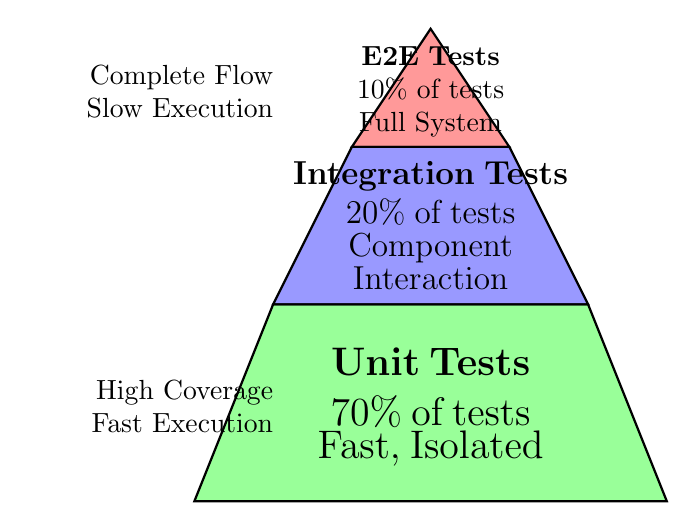
\begin{tikzpicture}
        % Draw pyramid layers
        \fill[green!40] (0,0) -- (6,0) -- (5,2.5) -- (1,2.5) -- cycle;
        \fill[blue!40] (1,2.5) -- (5,2.5) -- (4,4.5) -- (2,4.5) -- cycle;
        \fill[red!40] (2,4.5) -- (4,4.5) -- (3,6) -- cycle;

        % Labels with percentages
        \node[text width=4cm, align=center] at (3,1.2) {\Large \textbf{Unit Tests}\\70\% of tests\\Fast, Isolated};
        \node[text width=4cm, align=center] at (3,3.5) {\large \textbf{Integration Tests}\\20\% of tests\\Component Interaction};
        \node[text width=3cm, align=center] at (3,5.2) {\textbf{E2E Tests}\\10\% of tests\\Full System};

        % Borders
        \draw[thick] (0,0) -- (6,0) -- (5,2.5) -- (1,2.5) -- cycle;
        \draw[thick] (1,2.5) -- (5,2.5) -- (4,4.5) -- (2,4.5) -- cycle;
        \draw[thick] (2,4.5) -- (4,4.5) -- (3,6) -- cycle;

        % Coverage indicator
        \node[text width=3cm, align=right] at (-0.5,1.2) {High Coverage\\Fast Execution};
        \node[text width=3cm, align=right] at (-0.5,5.2) {Complete Flow\\Slow Execution};
    \end{tikzpicture}
    \caption{Testing Pyramid Strategy}
    \label{fig:testing-pyramid}
\end{figure}

\section{Unit Testing}
Unit tests form the foundation of the project's quality assurance. They are designed to test individual functions or components in isolation.
\begin{itemize}
    \item \textbf{Focus}: The primary focus of unit testing is on the business logic within the \texttt{internal/service} layer. This includes testing functions related to user creation, password hashing, JWT generation and validation, and manga data processing.
    \item \textbf{Mocking}: To achieve isolation, dependencies such as the database repository are mocked. This is done using interfaces. For example, the service layer depends on a \texttt{Repository} interface, and for testing, a mock implementation of this interface is provided that returns predefined data or errors without making an actual database call.
    \item \textbf{Examples}:
    \begin{itemize}
        \item An authentication test verifies that a correct password returns a valid JWT, while an incorrect password returns an error.
        \item A password hashing test ensures that the \texttt{bcrypt} hashing and comparison functions work as expected.
        \item A validation test confirms that input data (e.g., for user registration) is correctly validated and that appropriate errors are returned for invalid data.
    \end{itemize}
\end{itemize}

\section{Integration Testing}
Integration tests are used to verify the interaction between different parts of the system.
\begin{itemize}
    \item \textbf{API Flow}: A key focus of integration testing is the HTTP API. These tests start a real instance of the Gin server with a test database (either an in-memory SQLite database or a temporary file). HTTP requests are then made to the running server, and the responses (status code, headers, and body) are verified. This ensures that the entire flow—from routing and middleware to handlers, services, and the database—works correctly.
    \item \textbf{Protocol Interaction}: Integration tests also verify the functionality of the other protocol servers. For example:
    \begin{itemize}
        \item A TCP integration test involves a test client connecting to the TCP Sync Server, sending a progress update, and verifying that the update is correctly broadcast.
        \item A WebSocket test connects a client, sends and receives chat messages through the hub, and verifies that messages are routed to the correct room.
    \end{itemize}
\end{itemize}

\section{Performance Analysis}
While formal, extensive benchmarking is beyond the scope of this academic project, basic performance analysis was conducted to ensure the servers can handle a reasonable load.
\begin{itemize}
    \item \textbf{Load Testing Tools}: Standard tools like \texttt{wrk} or \texttt{ab} (Apache Benchmark) were used to send a high volume of concurrent requests to the HTTP API endpoints to measure response times and server throughput.
    \item \textbf{Concurrency}: Go's built-in race detector (\texttt{go test -race}) was used during testing to identify and fix potential race conditions in the concurrent code, particularly in the TCP and WebSocket servers where multiple goroutines share state.
    \item \textbf{Results}: The analysis confirmed that the lightweight nature of goroutines allows the servers to handle hundreds of concurrent connections with minimal memory overhead. The Gin framework's performance proved to be excellent, with API response times remaining low even under moderate load.
\end{itemize}% --- Chapter 6 ---\chapter{Conclusion and Future Work}

\section{Conclusion}
The MangaHub project successfully demonstrates the practical implementation and integration of five distinct network protocols to create a functional and cohesive manga tracking application. By leveraging the Go programming language and its powerful concurrency features, the project effectively showcases how HTTP, TCP, UDP, WebSocket, and gRPC can be used to solve real-world problems in a distributed system. The resulting application provides users with a comprehensive tool to manage their manga library, synchronize reading progress in real-time, receive instant notifications, and engage with a community, thereby achieving all the primary objectives set out at the beginning of the project. The microservices-style architecture, clean code structure, and robust testing strategy further highlight modern software engineering best practices.

\section{Challenges and Solutions}
Throughout the development process, several challenges were encountered:
\begin{itemize}
    \item \textbf{Concurrency Management}: Implementing the TCP and WebSocket servers required careful management of concurrent connections and shared state. The initial implementations were prone to race conditions. This was solved by using Go's standard concurrency patterns, including channels for communication between goroutines and mutexes for protecting shared data structures like the client list in the WebSocket hub.
    \item \textbf{Protocol Integration}: Ensuring seamless interaction between the different protocol servers was complex. For instance, triggering a UDP notification required communication from the service layer, which is primarily accessed by the HTTP server. This was addressed by implementing a lightweight internal event system or using gRPC for efficient inter-service communication.
    \item \textbf{Authentication Across Services}: A unified authentication strategy was needed across multiple protocols (HTTP, TCP, WebSocket). The solution was to standardize on JWT. For TCP and WebSocket connections, the client sends the JWT as the first message after establishing a connection, allowing the server to authenticate the session.
\end{itemize}

\section{Future Enhancements}
While the current implementation meets all core requirements, there are several avenues for future work that could further enhance the MangaHub platform:
\begin{itemize}
    \item \textbf{Redis Caching}: To improve performance and reduce database load, a Redis cache could be introduced to store frequently accessed data, such as manga details or user sessions.
    \item \textbf{Scalability and Deployment}: For a production environment, the application could be containerized using Docker and orchestrated with Kubernetes for automated scaling, deployment, and management. A load balancer like Nginx could be used to distribute traffic among multiple instances of the API server.
    \item \textbf{Advanced Search}: The search functionality could be enhanced by integrating a dedicated search engine like Elasticsearch, which would provide more powerful full-text search and filtering capabilities.
    \item \textbf{Mobile Applications}: Native mobile applications for iOS and Android could be developed to provide a better user experience on mobile devices, communicating with the same backend services.
\end{itemize}

\section{Acknowledgment}
We would like to express our sincere gratitude to our instructors and peers at the International University for their guidance, support, and valuable feedback throughout the course of this project. Their insights were instrumental in shaping the final application.

% --- References ---
\begin{thebibliography}{10}

\bibitem{kurose2021}
Kurose, J. F., \& Ross, K. W. (2021). \textit{Computer Networking: A Top-Down Approach} (8th ed.). Pearson Education.

\bibitem{woodbeck2021}
Woodbeck, A. (2021). \textit{Network Programming with Go: Essential Skills for Using and Securing Networks}. No Starch Press.

\bibitem{websocket-rfc}
Fette, I., \& Melnikov, A. (2011). The WebSocket Protocol (RFC 6455). Internet Engineering Task Force. Retrieved from \url{https://datatracker.ietf.org/doc/html/rfc6455}

\bibitem{fielding2000}
Fielding, R. T. (2000). \textit{Architectural Styles and the Design of Network-based Software Architectures} [Doctoral dissertation, University of California, Irvine]. Retrieved from \url{https://www.ics.uci.edu/~fielding/pubs/dissertation/top.htm}

\bibitem{grpc-docs}
Google. (2023). gRPC Documentation: Introduction to gRPC. Retrieved from \url{https://grpc.io/docs/what-is-grpc/introduction/}

\bibitem{gin-docs}
Gin Web Framework. (2023). Gin Web Framework Documentation. Retrieved from \url{https://gin-gonic.com/docs/}

\bibitem{gorilla-websocket}
Gorilla Web Toolkit. (2023). Gorilla WebSocket Package Documentation. Retrieved from \url{https://pkg.go.dev/github.com/gorilla/websocket}

\bibitem{effective-go}
The Go Programming Language. (2023). Effective Go. Retrieved from \url{https://go.dev/doc/effective_go}

\bibitem{sqlite-docs}
SQLite Consortium. (2023). SQLite Documentation. Retrieved from \url{https://www.sqlite.org/docs.html}

\bibitem{jwt-rfc}
Internet Engineering Task Force (IETF). (2015). JSON Web Token (JWT) (RFC 7519). Retrieved from \url{https://datatracker.ietf.org/doc/html/rfc7519}

\end{thebibliography}

% --- Appendices ---
\appendix

\chapter{API Endpoints Reference}

\section*{Authentication Endpoints}
\begin{itemize}
    \item \texttt{POST /api/v1/auth/register} - Register new user
    \item \texttt{POST /api/v1/auth/login} - Login and receive JWT token
    \item \texttt{POST /api/v1/auth/logout} - Logout (client-side token removal)
    \item \texttt{POST /api/v1/auth/refresh} - Refresh access token
    \item \texttt{GET /api/v1/auth/me} - Get current user profile
\end{itemize}

\section*{Manga Endpoints}
\begin{itemize}
    \item \texttt{GET /api/v1/manga} - List manga (paginated)
    \item \texttt{GET /api/v1/manga/:id} - Get manga details
    \item \texttt{POST /api/v1/manga} - Create manga (admin only)
    \item \texttt{PUT /api/v1/manga/:id} - Update manga (admin only)
    \item \texttt{DELETE /api/v1/manga/:id} - Delete manga (admin only)
    \item \texttt{GET /api/v1/manga/search} - Search manga by title/author
\end{itemize}

\section*{Library Endpoints}
\begin{itemize}
    \item \texttt{GET /api/v1/library} - Get user's library
    \item \texttt{POST /api/v1/library/:mangaId} - Add manga to library
    \item \texttt{DELETE /api/v1/library/:mangaId} - Remove manga from library
    \item \texttt{GET /api/v1/library/stats} - Get library statistics
\end{itemize}

\section*{Progress Endpoints}
\begin{itemize}
    \item \texttt{GET /api/v1/progress} - Get all progress entries
    \item \texttt{GET /api/v1/progress/:mangaId} - Get progress for specific manga
    \item \texttt{PUT /api/v1/progress/:mangaId} - Update reading progress
    \item \texttt{DELETE /api/v1/progress/:mangaId} - Clear progress
\end{itemize}

\section*{Health \& Utility}
\begin{itemize}
    \item \texttt{GET /health} - Server health check
    \item \texttt{GET /api/v1/version} - API version information
\end{itemize}

\textbf{Note}: All protected endpoints require \texttt{Authorization: Bearer <token>} header. Query parameters for pagination: \texttt{?page=1\&limit=20}. Search supports: \texttt{?search=keyword\&genre=action\&status=ongoing}.

\chapter{Database Schema}

\section*{Entity-Relationship Diagram}

\subsection*{USERS (Primary Entity)}
\begin{itemize}
    \item \texttt{id} (PK): UUID
    \item \texttt{username}: String, Unique
    \item \texttt{email}: String, Unique
    \item \texttt{password\_hash}: String
    \item \texttt{created\_at}: Timestamp
    \item \texttt{updated\_at}: Timestamp
\end{itemize}

\subsection*{MANGA (Primary Entity)}
\begin{itemize}
    \item \texttt{id} (PK): UUID
    \item \texttt{title}: String
    \item \texttt{author}: String
    \item \texttt{artist}: String
    \item \texttt{genres}: JSON Array
    \item \texttt{status}: Enum(ongoing, completed, hiatus)
    \item \texttt{total\_chapters}: Integer
    \item \texttt{description}: Text
    \item \texttt{cover\_image\_url}: String
    \item \texttt{created\_at}: Timestamp
    \item \texttt{updated\_at}: Timestamp
\end{itemize}

\subsection*{USER\_PROGRESS (Junction Entity)}
\begin{itemize}
    \item \texttt{user\_id} (PK, FK): References USERS(id)
    \item \texttt{manga\_id} (PK, FK): References MANGA(id)
    \item \texttt{current\_chapter}: Integer
    \item \texttt{current\_page}: Integer
    \item \texttt{status}: Enum(reading, completed, plan\_to\_read, dropped)
    \item \texttt{rating}: Integer (1-10)
    \item \texttt{notes}: Text
    \item \texttt{updated\_at}: Timestamp
\end{itemize}

\subsection*{Relationships}
\begin{itemize}
    \item USERS (1) $\leftrightarrow$ (M) USER\_PROGRESS: One user has many progress entries
    \item MANGA (1) $\leftrightarrow$ (M) USER\_PROGRESS: One manga tracked by many users
    \item USERS (1) $\leftrightarrow$ (M) USER\_LIBRARY: One user has many library entries
    \item MANGA (1) $\leftrightarrow$ (M) USER\_LIBRARY: One manga in many users' libraries
\end{itemize}

\subsection*{Database Indexes}
\begin{itemize}
    \item \texttt{idx\_manga\_title} ON manga(title)
    \item \texttt{idx\_manga\_author} ON manga(author)
    \item \texttt{idx\_user\_progress\_updated} ON user\_progress(updated\_at)
    \item \texttt{idx\_users\_username} ON users(username)
    \item \texttt{idx\_users\_email} ON users(email)
\end{itemize}

\chapter{Protocol Message Examples}

\section*{TCP Protocol Messages}

\textbf{Authentication:}
\begin{lstlisting}[language=json]
{"type":"auth","token":"eyJhbGci..."}
\end{lstlisting}

\textbf{Progress Update (Client → Server):}
\begin{lstlisting}[language=json]
{"type":"progress_update","manga_id":"manga-123",
 "current_chapter":42,"current_page":15}
\end{lstlisting}

\textbf{Progress Broadcast (Server → All User's Clients):}
\begin{lstlisting}[language=json]
{"type":"progress_update","user_id":"user-456",
 "manga_id":"manga-123","current_chapter":42,
 "current_page":15,"timestamp":"2025-01-15T10:30:00Z"}
\end{lstlisting}

\section*{UDP Protocol Messages}

\textbf{Subscribe to Notifications:}
\begin{lstlisting}[language=json]
{"type":"subscribe","user_id":"user-123",
 "manga_ids":["manga-456","manga-789"]}
\end{lstlisting}

\textbf{Chapter Release Notification:}
\begin{lstlisting}[language=json]
{"type":"chapter_release","manga_id":"manga-456",
 "manga_title":"One Piece","chapter":1100,
 "release_date":"2025-01-15"}
\end{lstlisting}

\section*{WebSocket Protocol Messages}

\textbf{Join Room:}
\begin{lstlisting}[language=json]
{"type":"join","room":"manga-456"}
\end{lstlisting}

\textbf{Chat Message:}
\begin{lstlisting}[language=json]
{"type":"message","room":"manga-456",
 "content":"This chapter was amazing!"}
\end{lstlisting}

\textbf{User Joined Notification:}
\begin{lstlisting}[language=json]
{"type":"user_joined","room":"manga-456",
 "username":"alice","user_count":15}
\end{lstlisting}

\end{document}
